\documentclass[10pt]{beamer}
\usepackage{xcolor}

% ------------------------------------------------------------------------
% Carga de tu preámbulo personalizado (preamble.tex)
% Asegúrate de tenerlo en la misma carpeta.
% ------------------------------------------------------------------------
\usetheme[progressbar=frametitle]{metropolis}
\usepackage{appendixnumberbeamer}
\usepackage{fancyvrb}
\usepackage{booktabs}
\usepackage[scale=2]{ccicons}
\usepackage{pgfplots}
\usepgfplotslibrary{dateplot}
\usepackage{type1cm}
\usepackage{lettrine}
\usepackage{ragged2e}
\usepackage{xspace}
\newcommand{\themename}{\textbf{\textsc{metropolis}}\xspace}
\usepackage{graphicx} % Allows including images
\usepackage{booktabs} % Allows the use of \toprule, \midrule and \bottomrule in tables
\usepackage[utf8]{inputenc} %solucion del problema de los acentos.
\usepackage{xcolor}
\definecolor{LightGray}{gray}{0.9}

\usepackage{minted}
\usemintedstyle{tango}
\newcommand{\mypyfile}[1]{\inputminted[linenos=true, fontsize=\footnotesize, frame=lines, framesep=5\fboxrule,framerule=1pt]{python}{#1}}

\setminted[python]{breaklines,frame=lines,framesep=2mm,baselinestretch=1.2,bgcolor=LightGray,linenos, fontsize=\footnotesize} % obeytabs=true, tabsize=2, showtabs=true}

%%%%%%%%%%%%%%%%%%%%%%%%%%%%%%%%%%%%%%%%%%%%%%%%%%%%%%%%%%%%%%%%%%%%%%%%%%%%%%%%%%%%%%
\setbeamercolor{progress bar}{fg=blue!50!black,bg=white!50!black}
\setbeamercolor{title separator}{fg=red!50!black,bg=white!50!black}
\setbeamercolor{frametitle}{fg=white!80!black,bg=red!50!black}
\title[PCFI161]{Programaci\'on para F\'isica y Astronom\'ia}
\subtitle{Departamento de Física.}

\newcommand{\myfront}{
\author[PCFI161]{Corodinadora: C Loyola \\ Profesoras/es C Loyola / C Femenías / Y Navarrete / C Ruiz}
\institute[UNAB]{Universidad Andrés Bello}
\date{Primer Semestre 2025}
}

\titlegraphic{%
  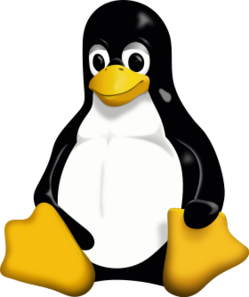
\includegraphics[width=.08\textwidth]{logo-tux.png}\hfill
  
\includegraphics[width=.3\textwidth]{logo-unab.png}\hfill
  
\includegraphics[width=.08\textwidth]{logo-python.png}
}

\makeatletter
\setbeamertemplate{title page}{
  \begin{minipage}[b][\paperheight]{\textwidth}
    \vfill%
    \ifx\inserttitle\@empty\else\usebeamertemplate*{title}\fi
    \ifx\insertsubtitle\@empty\else\usebeamertemplate*{subtitle}\fi
    \usebeamertemplate*{title separator}
    \ifx\beamer@shortauthor\@empty\else\usebeamertemplate*{author}\fi
    \ifx\insertdate\@empty\else\usebeamertemplate*{date}\fi
    \ifx\insertinstitute\@empty\else\usebeamertemplate*{institute}\fi
    \vfill
    \ifx\inserttitlegraphic\@empty\else\inserttitlegraphic\fi
    \vspace*{1cm}
  \end{minipage}
}
\makeatother


\makeatletter
\setlength{\metropolis@titleseparator@linewidth}{2pt}
\setlength{\metropolis@progressonsectionpage@linewidth}{2pt}
\setlength{\metropolis@progressinheadfoot@linewidth}{2pt}
\makeatother


\begin{document}

% ------------------------------------------------------------------------
% Portada de la Presentación
% ------------------------------------------------------------------------
\myfront{}

% ------------------------------------------------------------------------
% Slide 1: Título de la Sesión
% ------------------------------------------------------------------------
\begin{frame}
  \titlepage
  % Por ejemplo:
  % \title{Semana 4 - Sesión 1 (Sesión 7): Funciones en Python, Módulos y Paquetes}
\end{frame}

% ------------------------------------------------------------------------
% Slide 2: Índice / Tabla de contenidos
% ------------------------------------------------------------------------
\begin{frame}
  \frametitle{Resumen - Semana 3, Sesión 1 (Sesión 5)}
  \tableofcontents
\end{frame}

% ------------------------------------------------------------------------
% Configuración de bloques
% ------------------------------------------------------------------------
\metroset{block=fill}

% ----------------------------------------------------------------------------------------
% SECCIÓN 1: Introducción y Repaso de la Sesión Anterior
% ----------------------------------------------------------------------------------------
\section{Repaso y Contexto}

% ------------------------------------------------------------------------
% Slide 3: Recapitulación de la Sesión 6
% ------------------------------------------------------------------------
\begin{frame}{Recapitulación de la Sesión Anterior (Sesión 5)}
  \begin{itemize}
    \item \textbf{Semana 3, Sesión 1 (Sesión 5)} se centró en:
      \begin{itemize}
        \item Laboratorio práctico con estructuras de control (\texttt{if}, \texttt{while}).
        \item Problemas tipo: “Adivina el número”, “Calculadora de Calificaciones”, “Movimiento Discreto”.
        \item Manejo de validaciones, contadores y salidas controladas de bucles.
      \end{itemize}
      \textbf{Ejemplo}: {\texttt{\textcolor{blue}{def f(x): x=10}}} — la variable {\texttt{\textcolor{blue}{x}}} vive solo en {\texttt{\textcolor{blue}{f(x)}}}.
  \end{itemize}
\end{frame}

% ------------------------------------------------------------------------
% Slide 4: Objetivos de la Sesión 7
% ------------------------------------------------------------------------
\begin{frame}{Objetivos de la Sesión 5}
  \begin{itemize}
    \item \textbf{Comprender} la sintaxis y concepto de funciones en Python (\texttt{def}, parámetros, \texttt{return}).
    \item \textbf{Explorar} cómo organizar código en módulos y paquetes simples.
    \item \textbf{Aplicar} estos conceptos a pequeños proyectos para mejorar reutilización y claridad.
    \item \textbf{Conectar} funciones con los temas previos (estructuras de control, manejo de datos, etc.).
  \end{itemize}
\end{frame}

% ----------------------------------------------------------------------------------------
% SECCIÓN 2: Funciones en Python
% ----------------------------------------------------------------------------------------
\section{Funciones en Python}

% ------------------------------------------------------------------------
% Slide 5: Definición y Motivación
% ------------------------------------------------------------------------
\begin{frame}{¿Por qué usar Funciones?}
  \begin{itemize}
    \item \textbf{Reutilización de Código}: evitar escribir la misma lógica en múltiples lugares.
    \item \textbf{Organización}: encapsular tareas específicas en “cajas negras”.
    \item \textbf{Legibilidad}: el nombre de la función describe la operación que realiza.
    \item \textbf{Mantenibilidad}: cambiar la lógica en un solo lugar (la definición de la función).
  \end{itemize}
\end{frame}

% ------------------------------------------------------------------------
% Slide 6: Sintaxis de una Función
% ------------------------------------------------------------------------
\begin{frame}[fragile]{Sintaxis Básica de Funciones en Python}
\begin{minted}{python}
def nombre_de_funcion(param1, param2, ...):
    """
    Documentación opcional (docstring).
    Explica qué hace la función, los parámetros y el retorno.
    """
    # bloque de código
    # opcionalmente retornar un valor
    return resultado
\end{minted}

\begin{itemize}
  \item \textbf{Parámetros}: valores de entrada que la función utiliza.
  \item \textbf{return}: finaliza la función y opcionalmente devuelve un valor.
  \item \textbf{Mejor práctica}: Usar nombres descriptivos para parámetros y funciones.
\end{itemize}
\end{frame}

% ------------------------------------------------------------------------
% Slide 7: Ejemplo de Función Sencilla
% ------------------------------------------------------------------------
\begin{frame}[fragile]{Ejemplo: Función para Calcular el Área de un Círculo}
\begin{minted}{python}
import math

def area_circulo(radio):
    """
    Retorna el área de un círculo de radio 'radio'.
    Formula: pi * r^2
    """
    area = math.pi * (radio**2)
    return area

# Uso de la función
r = 5
a = area_circulo(r)
print("El área del círculo es:", a)
\end{minted}

\begin{itemize}\tiny
  \item \textbf{Encapsulamos} la operación en \texttt{area\_circulo}.
  \item \textbf{Parámetro} \texttt{radio}.
  \item \textbf{Retorno} con \texttt{return area}.
\end{itemize}
\end{frame}

% ----------------------------------------------------------------------------------------
% SECCIÓN 3: Parámetros, Retornos y Alcance
% ----------------------------------------------------------------------------------------
\section{Parámetros y Alcance}

% ------------------------------------------------------------------------
% Slide 8: Tipos de Parámetros (Posicionales, Opcionales)
% ------------------------------------------------------------------------
\begin{frame}[fragile]{Parámetros Posicionales y Opcionales}
\begin{minted}{python}
def calcular_salario(base, horas_extra=0):
    """Calcula salario sumando base + 2000 por hora extra"""
    return base + 2000 * horas_extra

s1 = calcular_salario(50000)      # horas_extra por defecto: 0
s2 = calcular_salario(50000, 3)   # 3 horas extra
print(s1, s2)
\end{minted}
\begin{itemize}
  \item \textbf{Parámetros con valor por defecto} (ej. \texttt{horas\_extra=0}).
  \item \textbf{Posicionales}: deben ir en orden; \texttt{calcular\_salario(50000, 3)}.
  \item \textbf{Keyword arguments}: \texttt{calcular\_salario(base=50000, horas\_extra=3)}.
\end{itemize}
\end{frame}

% ------------------------------------------------------------------------
% Slide 9: Alcance de Variables (Scope)
% ------------------------------------------------------------------------
\begin{frame}{Scope o Alcance de Variables}
  \begin{itemize}
    \item \textbf{Local}: Variables definidas dentro de la función solo existen dentro de ella.
    \item \textbf{Global}: Variables definidas fuera de cualquier función son accesibles dentro, pero no se recomienda modificarlas sin razón.
    \item \textbf{Mejor práctica}: Mantener funciones “puras”, evitando depender de variables globales.
  \end{itemize}
  \vspace{0.2cm}
  \textbf{Ejemplo}: {\texttt{\textcolor{blue}{def f(): x=10}}} — la variable {\texttt{\textcolor{blue}{x}}} vive solo en {\texttt{\textcolor{blue}{f()}}}.
\end{frame}

% ------------------------------------------------------------------------
% Slide 10: Ejemplo de Conflicto Global vs Local
% ------------------------------------------------------------------------
\begin{frame}[fragile]{Conflicto Global vs Local}
\begin{minted}{python}
x = 5  # global

def foo():
    x = 10  # local
    print("Dentro de foo, x =", x)

foo()
print("Fuera de foo, x =", x)
\end{minted}
\begin{itemize}
  \item Impresiones:
    \begin{itemize}
      \item “Dentro de foo, x = 10”
      \item “Fuera de foo, x = 5”
    \end{itemize}
  \item \textbf{Evitar confusiones} usando nombres significativos y parámetros claros.
\end{itemize}
\end{frame}

% ----------------------------------------------------------------------------------------
% SECCIÓN 4: Módulos y Paquetes
% ----------------------------------------------------------------------------------------
\section{Módulos y Paquetes}

% ------------------------------------------------------------------------
% Slide 11: ¿Qué es un Módulo?
% ------------------------------------------------------------------------
\begin{frame}{¿Qué es un Módulo en Python?}
  \begin{itemize}
    \item Un \textbf{módulo} es un archivo \texttt{.py} que contiene definiciones de funciones, variables y clases.
    \item \textbf{Ventaja}: podemos importar este archivo desde otros scripts y reutilizar el código.
    \item \textbf{Ejemplo}: Crear un archivo \texttt{mifunciones.py} con varias funciones y luego:
    \[
      \texttt{import mifunciones}
    \]
  \end{itemize}
\end{frame}

% ------------------------------------------------------------------------
% Slide 12: Ejemplo de Módulo Sencillo
% ------------------------------------------------------------------------
\begin{frame}[fragile]{Ejemplo de Módulo: \texttt{mifunciones.py}}
\begin{minted}{python}
# mifunciones.py

def suma(a, b):
    return a + b

def resta(a, b):
    return a - b
\end{minted}
\vspace{0.3cm}
\textbf{Uso en otro archivo}:
\begin{minted}[
  frame=lines,
  framesep=2mm,
  fontsize=\footnotesize,
  bgcolor=LightGray
]{python}
import mifunciones

print(mifunciones.suma(3, 4))
print(mifunciones.resta(10, 2))
\end{minted}
\end{frame}

% ------------------------------------------------------------------------
% Slide 13: \texttt{from ... import ...}
% ------------------------------------------------------------------------
\begin{frame}[fragile]{Importaciones Específicas}
\begin{minted}{python}
from mifunciones import suma

resultado = suma(5, 7)
print(resultado)
\end{minted}
\begin{itemize}
  \item Trae solo la función \texttt{suma} del módulo.
  \item \textbf{Cuidado}: peligro de colisiones de nombre (si hay otra \texttt{suma}).
  \item \texttt{from mifunciones import *} trae todo, también puede causar conflictos.
\end{itemize}
\end{frame}

% ------------------------------------------------------------------------
% Slide 14: Paquetes (Carpetas con \_\_init\_\_.py)
% ------------------------------------------------------------------------
\begin{frame}{Paquetes en Python}
  \begin{itemize}
    \item Un \textbf{paquete} es una carpeta que contiene un archivo \texttt{\_\_init\_\_.py} y varios módulos \texttt{.py}.
    \item Estructura típica:  mypackage/modulo1.py  mypackage/modulo1.py
    \item Para usarlo: \texttt{import mipaquete.modulo1}.
  \end{itemize}
  \textbf{Uso}: Organizar proyectos grandes en submódulos lógicamente separados.
\end{frame}

% ----------------------------------------------------------------------------------------
% SECCIÓN 5: Ejercicios Guiados
% ----------------------------------------------------------------------------------------
\section{Ejercicios Guiados}

% ------------------------------------------------------------------------
% Slide 18: Ejercicio 1 - Función con Condicionales y Bucle
% ------------------------------------------------------------------------
\begin{frame}{Ejercicio 1: \hfill \textcolor{red}{$\clubsuit$} \\ 
Suma Condicional}
  \begin{block}{Enunciado}
    Crear una función que reciba dos números y realice lo siguiente:
    \begin{itemize}
      \item Si ambos números son positivos, retornar su suma.
      \item Si uno de los números es negativo, retornar su división.
      \item Si ambos números son negativos, retornar su producto.
    \end{itemize}
  \end{block}
  \textbf{Conceptos:} Uso de estructuras condicionales (\texttt{if}, \texttt{elif}, \texttt{else}).
\end{frame}

% ------------------------------------------------------------------------
% Slide 19: Ejercicio 2 - Clasificación con Ciclo
% ------------------------------------------------------------------------
\begin{frame}{Ejercicio 2: \hfill \textcolor{red}{$\clubsuit$} \\ 
Clasificación de Números}
  \begin{block}{Enunciado}
    Crear una función que reciba una lista de números y clasifique cada número como:
    \begin{itemize}
      \item Positivo.
      \item Negativo.
      \item Cero.
    \end{itemize}
    La función debe imprimir el resultado para cada número y retornar la cantidad de números positivos, negativos y ceros.
  \end{block}
  \textbf{Conceptos:} Uso de ciclos \texttt{for} y estructuras condicionales.
\end{frame}

% ------------------------------------------------------------------------
% Slide 20: Ejercicio 3 - Suma con Validación
% ------------------------------------------------------------------------
\begin{frame}{Ejercicio 3: \hfill \textcolor{red}{$\clubsuit$} \\ 
Suma de Números con Validación}
  \begin{block}{Enunciado}
    Crear una función que reciba un número entero \( n \) y realice lo siguiente:
    \begin{itemize}
      \item Solicitar al usuario \( n \) números enteros.
      \item Validar que cada número ingresado sea mayor que cero. Si no lo es, volver a solicitar el número.
      \item Retornar la suma de los \( n \) números ingresados.
    \end{itemize}
  \end{block}
  \textbf{Conceptos:} Uso de ciclos \texttt{while} y validaciones.
\end{frame}

% ------------------------------------------------------------------------
% Slide 21: Ejercicio 4 - Serie de Fibonacci
% ------------------------------------------------------------------------
\begin{frame}{Ejercicio 4: \hfill \textcolor{red}{$\clubsuit$} \\ 
Serie de Fibonacci}
  \begin{block}{Enunciado}
    Crear una función que reciba un número entero \( n \) y retorne los primeros \( n \) términos de la serie de Fibonacci.
    \begin{itemize}
      \item La serie de Fibonacci comienza con 0 y 1.
      \item Cada término siguiente es la suma de los dos anteriores.
    \end{itemize}
  \end{block}
  \textbf{Conceptos:} Uso de ciclos \texttt{for} y listas.
\end{frame}

% ------------------------------------------------------------------------
% Slide 22: Ejercicio 5 - Número Primo
% ------------------------------------------------------------------------
\begin{frame}{Ejercicio 5: \hfill \textcolor{red}{$\clubsuit$} \\ 
Verificación de Número Primo}
  \begin{block}{Enunciado}
    Crear una función que reciba un número entero y determine si es primo o no.
    \begin{itemize}
      \item Un número primo es divisible únicamente por 1 y por sí mismo.
      \item La función debe retornar \texttt{True} si el número es primo y \texttt{False} en caso contrario.
    \end{itemize}
  \end{block}
  \textbf{Conceptos:} Uso de ciclos \texttt{for} y estructuras condicionales.
\end{frame}


% ------------------------------------------------------------------------
% Slide 23: Solución 1 de Referencia - Suma Condicional
% ------------------------------------------------------------------------
\begin{frame}[fragile]{Solución 1 de Referencia: \hfill \textcolor{green}{$\checkmark$} \\ 
Suma Condicional}
\begin{minted}[fontsize=\tiny]{python}
def suma_condicional(a, b):
    """
    Realiza operaciones según los valores de a y b:
    - Si ambos son positivos, retorna su suma.
    - Si uno es negativo, retorna su división.
    - Si ambos son negativos, retorna su producto.
    """
    if a > 0 and b > 0:
        return a + b
    elif a < 0 and b < 0:
        return a * b
    else:
        return a / b

# Ejemplo de uso
resultado = suma_condicional(5, -3)
print("Resultado:", resultado)
\end{minted}
\textbf{Discusión:} ¿Qué sucede si \( b = 0 \) en la división? ¿Cómo manejar este caso?
\end{frame}

% ------------------------------------------------------------------------
% Slide 24: Solución 2 de Referencia - Clasificación con Ciclo
% ------------------------------------------------------------------------
\begin{frame}[fragile]{Solución 2 de Referencia: \hfill \textcolor{green}{$\checkmark$} \\ 
Clasificación de Números}
\begin{minted}[fontsize=\tiny]{python}
def clasificar_numeros(lista):
    """
    Clasifica números en positivos, negativos y ceros.
    Retorna la cantidad de cada tipo.
    """
    positivos = 0
    negativos = 0
    ceros = 0

    for num in lista:
        if num > 0:
            print(f"{num} es positivo")
            positivos += 1
        elif num < 0:
            print(f"{num} es negativo")
            negativos += 1
        else:
            print(f"{num} es cero")
            ceros += 1

    return positivos, negativos, ceros

# Ejemplo de uso
resultado = clasificar_numeros([3, -1, 0, 7, -5])
print("Positivos, Negativos, Ceros:", resultado)
\end{minted}
\textbf{Discusión:} ¿Cómo manejar listas vacías o valores no numéricos?
\end{frame}

% ------------------------------------------------------------------------
% Slide 25: Solución 3 de Referencia - Suma con Validación
% ------------------------------------------------------------------------
\begin{frame}[fragile]{Solución 3 de Referencia: \hfill \textcolor{green}{$\checkmark$} \\ 
Suma de Números con Validación}
\begin{minted}[fontsize=\tiny]{python}
def suma_con_validacion(n):
    """
    Solicita n números positivos al usuario y retorna su suma.
    Valida que cada número ingresado sea mayor que cero.
    """
    suma = 0
    contador = 0

    while contador < n:
        num = float(input(f"Ingrese el número {contador + 1}: "))
        if num > 0:
            suma += num
            contador += 1
        else:
            print("El número debe ser mayor que cero. Intente de nuevo.")

    return suma

# Ejemplo de uso
resultado = suma_con_validacion(3)
print("Suma total:", resultado)
\end{minted}
\textbf{Discusión:} ¿Cómo manejar entradas no numéricas o interrupciones del usuario?
\end{frame}

% ------------------------------------------------------------------------
% Slide 26: Solución 4 de Referencia - Serie de Fibonacci
% ------------------------------------------------------------------------
\begin{frame}[fragile]{Solución 4 de Referencia: \hfill \textcolor{green}{$\checkmark$} \\ 
Serie de Fibonacci}
\begin{minted}[fontsize=\tiny]{python}
def fibonacci(n):
    """
    Retorna los primeros n términos de la serie de Fibonacci.
    """
    if n <= 0:
        return []
    elif n == 1:
        return [0]
    elif n == 2:
        return [0, 1]

    serie = [0, 1]
    for i in range(2, n):
        siguiente = serie[-1] + serie[-2]
        serie.append(siguiente)

    return serie

# Ejemplo de uso
resultado = fibonacci(10)
print("Serie de Fibonacci:", resultado)
\end{minted}
\textbf{Discusión:} ¿Cómo optimizar para valores grandes de \( n \)?
\end{frame}

% ------------------------------------------------------------------------
% Slide 27: Solución 5 de Referencia - Número Primo
% ------------------------------------------------------------------------
\begin{frame}[fragile]{Solución 5 de Referencia: \hfill \textcolor{green}{$\checkmark$} \\ 
Verificación de Número Primo}
\begin{minted}[fontsize=\tiny]{python}
def es_primo(num):
    """
    Determina si un número es primo.
    Retorna True si es primo, False si no.
    """
    if num < 2:
        return False
    for i in range(2, num):
        if num % i == 0:
            return False
    return True

# Ejemplo de uso
resultado = es_primo(13)
print("¿Es primo?", resultado)
\end{minted}
\textbf{Discusión:} ¿Cómo manejar números negativos o muy grandes?
\end{frame}

% ----------------------------------------------------------------------------------------
% SECCIÓN 6: Actividad Práctica
% ----------------------------------------------------------------------------------------
\section{Actividad Práctica}

% ------------------------------------------------------------------------
% Slide 21: Actividad Extra 1 - Función Avanzada
% ------------------------------------------------------------------------
\begin{frame}{Actividad Extra 1: \hfill \textcolor{blue}{$\clubsuit$} \\
Función Avanzada}
  \begin{block}{Enunciado}
    Crear una función que calcule el factorial de un número de forma recursiva (que la función se llame a sí misma).
  \end{block}
  \textbf{Objetivo:} Aplicar recursión.
\end{frame}

% ------------------------------------------------------------------------
% Slide 22: Actividad Extra 2 - Módulo Personalizado
% ------------------------------------------------------------------------
\begin{frame}{Actividad Extra 2: \hfill \textcolor{blue}{$\clubsuit$} \\
Módulo Personalizado}
  \begin{block}{Enunciado}
    Crear un módulo con funciones para calcular el área y perímetro de figuras geométricas básicas (círculo, cuadrado, triángulo).
  \end{block}
  \textbf{Objetivo:} Modularizar el código y practicar importaciones.
\end{frame}

% ------------------------------------------------------------------------
% Slide 23: Actividad Extra 3 - Proyecto Integrador
% ------------------------------------------------------------------------
\begin{frame}{Actividad Extra 3: \hfill \textcolor{blue}{$\clubsuit$} \\
Proyecto Integrador}
  \begin{block}{Enunciado}
    Diseñar un programa que utilice funciones y módulos para resolver un problema práctico, como una calculadora científica básica.
  \end{block}
  \textbf{Objetivo:} Integrar conceptos de funciones, módulos y estructuras de control.
\end{frame}

% ------------------------------------------------------------------------
% Slide 17: Actividad - Organizándote con Módulos
% ------------------------------------------------------------------------
\begin{frame}{Actividad Extra 4: Creando Tus Módulos}
  \begin{itemize}
    \item \textbf{Objetivo}: Organizar funciones útiles en un módulo y probar su importación.
    \item \textbf{Instrucciones}:
      \begin{enumerate}
        \item Crea un archivo \texttt{utilidades.py} con al menos 3 funciones (ej. \texttt{factorial(n)}, \texttt{es\_primo(n)}, etc.).
        \item En un \textbf{notebook de Colab} o un script \texttt{main.py}, importa \texttt{utilidades} y prueba dichas funciones.
        \item (Opcional) Añade una cuarta función con un \textbf{parámetro por defecto} (\texttt{def hola\_mundo(nombre="Mundo")}, etc.).
      \end{enumerate}
  \end{itemize}
  \textbf{Sugerencia}: Comenta tu código y explica la lógica de cada función.
  \textbf{Reflexión}: ¿Cómo ayuda la modularización a proyectos más grandes?
\end{frame}

% ------------------------------------------------------------------------
% Slide 18: Trabajo en Clase
% ------------------------------------------------------------------------
\begin{frame}{Trabajo Colaborativo}
  \begin{itemize}
    \item Formar \textbf{parejas o tríos}.
    \item Diseñar \textbf{un pequeño módulo} de funciones:
      \begin{itemize}
        \item Matemáticas, Estadística básica, Conversión de unidades, etc.
      \end{itemize}
    \item Utilizar dichas funciones en \textbf{otro script} o \textbf{notebook}.
    \item \textbf{Opcional}: Explorar la creación de una carpeta con \texttt{\_\_init\_\_.py} para armar un paquete simple.
  \end{itemize}
\end{frame}

% ------------------------------------------------------------------------
% Slide 19: Dudas y Apoyo
% ------------------------------------------------------------------------
\begin{frame}{Espacio para Dudas y Apoyo}
  \begin{itemize}
    \item ¿Problemas al importar el módulo en Colab?
    \item ¿Cómo organizar los archivos en Google Drive?
    \item ¿Errores de \texttt{ModuleNotFoundError}?
  \end{itemize}
  \vspace{0.2cm}
  \textbf{Consulta en voz alta o pide ayuda a tus compañeros.}
\end{frame}

% ------------------------------------------------------------------------
% Slide 22: Retroalimentación y Observaciones
% ------------------------------------------------------------------------
\begin{frame}{Retroalimentación}
  \begin{itemize}
    \item ¿Se entendió la \textbf{separación} entre la lógica (en un módulo .py) y el código principal?
    \item ¿Ventajas de tener todo en un solo archivo vs. múltiples módulos?
    \item ¿Dudas sobre parámetros y valores por defecto?
  \end{itemize}
\end{frame}

% ----------------------------------------------------------------------------------------
% SECCIÓN 6: Conclusiones y Próximos Pasos
% ----------------------------------------------------------------------------------------
\section{Conclusiones}

% ------------------------------------------------------------------------
% Slide 23: Conclusiones de la Sesión
% ------------------------------------------------------------------------
\begin{frame}{Conclusiones de la Sesión 7}
  \begin{itemize}
    \item Apreciamos la \textbf{modularización} del código para mejor legibilidad y mantenimiento.
    \item Vimos \textbf{funciones}: sintaxis \texttt{def}, parámetros, \texttt{return}, docstring.
    \item Exploramos la creación de \textbf{módulos} y su importación en otros scripts o notebooks.
    \item Ahora estamos preparados para proyectos más grandes y ordenados.
  \end{itemize}
\end{frame}

% ------------------------------------------------------------------------
% Slide 24: Próximos Temas
% ------------------------------------------------------------------------
\begin{frame}{Próximos Temas}
  \begin{itemize}
    \item \textbf{Sesion 8 (Semana 4)}: Continuaremos con el uso de módulos y paquetes, y profundizaremos en el uso de \texttt{pip} y librerías externas.
    \item \textbf{Tarea sugerida}:
      \begin{itemize}
        \item Crear un pequeño proyecto con un paquete \texttt{mipaquete/} y varios módulos (ej. \texttt{mipaquete/calculos.py}, \texttt{mipaquete/utiles.py}, etc.).
        \item Probar importarlos y usarlos en un script principal.
      \end{itemize}
  \end{itemize}
\end{frame}

% ------------------------------------------------------------------------
% Slide 25: Cierre de la Sesión
% ------------------------------------------------------------------------
\begin{frame}
  \huge{\centerline{¡Gracias y hasta la próxima sesión!}}
  \vspace{0.5cm}
  \normalsize
  \begin{itemize}
    \item Guarda tus \textbf{notebooks} y archivos \texttt{.py} en Google Drive.
    \item Explora la documentación oficial de Python (sobre \textbf{funciones} y \textbf{módulos}).
    \item ¡Sigue practicando!
  \end{itemize}
\end{frame}

\end{document}

